% FleCSI Data Requirements: Introduction
\section{Introduction}
The goal of this Research Note is to identify requirements for the FleCSI data model.
Additional documentation will discuss design options, testing, and so on.

There are a number of different areas of data management:
\begin{enumerate}
\item data associated with mesh elements (so-called \emph{mesh fields});
\item particle data;
\item data associated with physical models (equation of state, for example);
\item simulation state data that is set at launch time, but does not change afterward (physics configuration, for example);
\item simulation state data that varies during the run (cycle number, for instance).
\end{enumerate}

A field can be thought of as a relation from a set of mesh entities (such as cell centers or edges) to some other set of objects (such as double precision numbers or geometric vectors).
It is useful to distinguish between the Field, which is the abstract object or mapping, and the FieldData, the actual velocity in cells 1,2,3, etc.
Field and FieldData requirements are discussed in \S\ref{FieldRequirementsSec}.

Physical model data is (typically) in tabular form, and represents the results of (usually) expensive constitutive modeling.
The use cases and requirements for physical model data are covered in \S\ref{PhysicalModelRequirementsSec}.

Static and mutable simulation data include control data, as well as physical and computational configuration data.
These use cases and requirements are covered in \S\ref{SimConstRequirementsSec} (constant) and \S\ref{SimMutableRequirementsSec} (mutable).

\subsection{FleCSI Programming Model}

The computing model that we have in mind features the elements summarized in Table~\ref{flecsi_actors_table}.
\begin{table}[hbt]
\begin{tabular}{l p{5 in}}
\toprule
Processing Element & Description \\
\midrule
Application & (Runtime?): instantiates DataStore and objects that interact with it;\\
DataStore &  manages fields, field data (as well as other types of data not directly associated with mesh elements)\\
Package &  namespace for tasks, typically associated with a physics operator, provides Tasks and one or more Drivers;\\
Driver &  Shares data between tasks and , can interact with the DataStore to coordinate \\
Task &  Coordinates kernels to accomplish a task. Can interact with the DataStore, can operate on field data passed to it by its Driver; tasks can interact with the data store to obtain temporary state, make state visible to the application.\\
Kernel &  stateless computation, it operates on the data provided to it by its task; kernels do not interact with DataStore.\\
\bottomrule
\end{tabular}
\centering
\parbox{5in}{\caption{Actors in the FleCSI computing model.\label{flecsi_actors_table}}}
% \stepcounter{useTable}
\end{table}

\subsubsection{Kernel}
A kernel is pure function that accomplishes a single, well--defined job.
In physics terms, a kernel computes some interesting quantity from its inputs and returns that quantity as its output.
At first, think of a kernel as code to compute a single thing---that is, one number.
The application of the kernel over a larger collection, such as a data field, will be performed by something else.

Pure in this context means that the invocation of the kernel can be replaced by the return value of the kernel.
This means that the kernel cannot do many things.
A kernel cannot communicate; it cannot print something to the screen; it cannot store data that would affect future invocations.
It's meant to be a function in a very mathematical sense: it's a machine whose behavior is completely dictated by its inputs.

Note that this does not preclude a kernel from being a callable object (in one of C++'s more egregious parochialisms, a ``functor'').
It just means that invoking the kernel cannot change the state of the object.
Thus, one could parameterize the kernel object at construction time, then leave it alone.
Syntactically, this is equivalent to declaring the call operator const, for example:
\begin{verbatim}
struct Kernel58
{
    ...
    ReturnT operator()(InputT i, ...) const {...}
    ...
};
\end{verbatim}

\subsubsection{Task}
A Task coordinates one or more Kernels to accomplish a more complicated undertaking.
For example, a Task might apply a kernel to each element of a Field.
A larger scale Task would coordinate multiple kernels.

\subsubsection{Driver}
A driver is a task that holds special status as one of a few principle entry points of a package.

\subsection{Data Policies for FleCSI Programming Model}
Policy choices will create requirements for the various elements that will need to be reflected in the design.
Core policy decisions include access and lifecycle.

Policies also need to distinguish between the various roles that tasks play.
For example, data mutating tasks need to be very careful about access to data.
Non-mutating tasks, such as monitoring, can probably be given freer access.

Programmers also need to be careful about data access.
Accessing data from the DataStore essentially limits the reusability of a piece of code.
Such accesses should be carefully encapsulated.

\subsubsection{Possible Policy 1: `The-Hell-With-It'}
One policy is everyone gets everything at any time.
The advantage of this approach is expedience: it requires no thought.
The disadvantage of this approach is that in effect, it turns the DataStore into a colossal common block.
Though a historically popular choice, The-Hell-With-It policy is maintenace nightmare, and it fundamentally obscures the physics protocol (operator coupling).
This policy would definitely be a Last Generation Code choice.


\subsubsection{Possible Policy 2: Limited Hierarchy Policy}

Another policy would seek to enforce the usual hierarhical approach to program organization.
In this approach, data objects can only be passed downward, one level at a time.

\begin{figure}[ht]
\centering
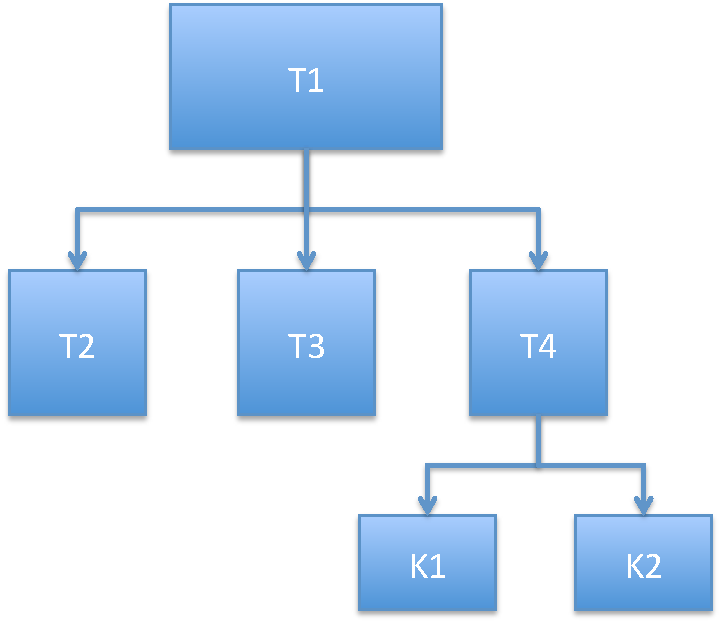
\includegraphics[scale=0.5]{figures/SimpleHierarchy.pdf}
\parbox{6in}{\caption{A simple processing network.\label{simple_hierarchy_fig}}}
\end{figure}

In more detail, the rules of this policy are:
\begin{enumerate}
\item no data is passed (taken) laterally,
\item passing data between levels of the hierarchy must be explicit,
\item that lower elements use data objects provided by the higher levels,
\item that higher elements do not access objects created by lower elements,
\item and that lower elements do not use data objects from siblings.
\end{enumerate}

Refering to the diagram in Fig.~\ref{simple_hierarchy_fig}, we could immediately infer the following constraints:
\begin{enumerate}
\item T3 can use read/write data provided by T1;
\item T3 cannot use any data created by T2, nor any data provided by T1 to T2, unless T1 happens to provide that data to T3 as well;
\item T1 could not use data created by T3;
\item K2 could use data provided by T4;
\item The only way that K2 could use data provided by T1 would be if T4 explicitly relayed it to K2.
\end{enumerate}

